% !TEX root = task-1-3-5.tex
% Editable task bank. Append new BankTask blocks at the end of the document.
\documentclass[12pt,a4paper]{article}
\usepackage{physics-textbook}
\usepackage{graphicx,needspace}
\usetikzlibrary{decorations.pathmorphing}
\newif\ifShowSolutions
\ifdefined\TutorEdition
  \ShowSolutionstrue
\else
  \ShowSolutionsfalse % Change to \ShowSolutionstrue to display solutions.
\fi
\newcounter{banktask}
\newsavebox{\BankTaskBox}
\newcommand{\BankTaskContent}[3]{%
  \noindent\textbf{\thebanktask.}\quad #2\par
  \ifShowSolutions
    \Needspace{50mm}% Keep the solution heading with its opening text or diagram.
    #3\par
    \ifdefined\TutorEdition
      \ifcsname TutorSource#1\endcsname
        \nopagebreak\smallskip{\small\csname TutorSource#1\endcsname\par}%
      \fi
    \fi
  \fi
}
\newcommand{\BankTask}[3]{%
  \refstepcounter{banktask}\par\medskip
  \sbox{\BankTaskBox}{\begin{minipage}{\linewidth}%
    \BankTaskContent{#1}{#2}{#3}\end{minipage}}%
  \ifdim\dimexpr\ht\BankTaskBox+\dp\BankTaskBox\relax>\dimexpr\textheight-20mm\relax
    \Needspace{35mm}\BankTaskContent{#1}{#2}{#3}%
  \else
    \Needspace{\dimexpr\ht\BankTaskBox+\dp\BankTaskBox\relax}%
    \noindent\usebox{\BankTaskBox}\par
  \fi
  \medskip
}
\begin{document}
\BookSubsection{1.3.5}{Горизонтальный бросок}


% Source sdamgia-6505: https://phys-ege.sdamgia.ru/problem?id=6505
\BankTask{sdamgia-6505}{
\begin{center}
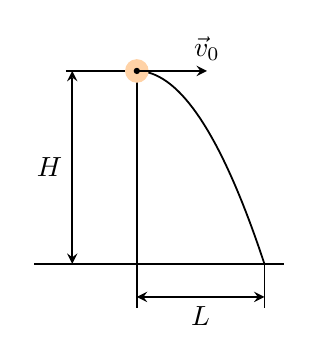
\begin{tikzpicture}[>=stealth,line width=.65pt]
\draw (-1.3,0)--(1.87,0);
\draw (0,-.56)--(0,2.45);
\draw (1.62,0)--(1.62,-.56);
\draw[<->] (-.82,0)--(-.82,2.45) node[midway,left]{$H$};
\draw (-.9,2.45)--(0,2.45);
\draw[<->] (0,-.42)--(1.62,-.42) node[midway,below]{$L$};
\draw[domain=0:1.62,samples=35,smooth,variable=\x] plot ({\x},{2.45*(1-(\x/1.62)^2)});
\fill[orange!35] (0,2.45) circle (.15);
\fill (0,2.45) circle (.04);
\draw[->] (0,2.45)--(0.89,2.45) node[above]{$\vec v_0$};
\end{tikzpicture}
\end{center}
Шарик, брошенный горизонтально с высоты $H$ с начальной скоростью $\upsilon _{0}$, за время $t$ пролетел в горизонтальном направлении расстояние $L$ (см. рис.). Что произойдет с временем полета и дальностью полета, если на этой же установке уменьшить начальную скорость шарика в $2$ раза? Сопротивлением воздуха пренебречь. 

Для каждой величины определите соответствующий характер ее изменения.

$1$. Увеличится.

$2$. Уменьшится.

$3$. Не изменится.

 

\begin{center}\small\renewcommand{\arraystretch}{1.25}\begin{tabular}{|p{0.450\linewidth}|p{0.450\linewidth}|}\hline
Время полета & Дальность полета\\\hline
 & \\\hline
\end{tabular}\end{center}
}{
\smallskip\noindent\textbf{Решение}\par
Время полета шарика определяется временем его падения и рассчитывается по формуле $t= \sqrt{\frac{2H}{g}} .$ Потому при уменьшении начальной скорости время полета не изменится. Дальность полета определяется начальной скоростью и временем полета тела: $L= v _0t,$ следовательно, при уменьшении начальной скорости в два раза дальность полета также уменьшится в два раза.

Ответ: $32$.
}

% Source sdamgia-6920: https://phys-ege.sdamgia.ru/problem?id=6920
\BankTask{sdamgia-6920}{
\begin{center}
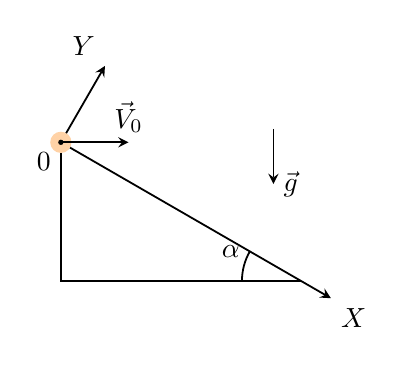
\begin{tikzpicture}[>=stealth,line width=.65pt]
\draw (0,0)--(0,-1.76)--(3.05,-1.76);
\draw[->] (0,0)--(3.43,-1.98) node[below right]{$X$};
\draw[->] (0,0)--(.56,.97) node[above left]{$Y$};
\draw (2.30,-1.76) arc[start angle=180,end angle=150,radius=.75] node[left] {$\alpha$};
\fill[orange!35] (0,0) circle (.135);
\fill (0,0) circle (.034);
\node[below left] at (0,0) {$0$};
\draw[->] (0,0)--(.86,0) node[above] {$\vec V_0$};
\draw[->] (2.70,.17)--(2.70,-.53) node[right] {$\vec g$};
\end{tikzpicture}
\end{center}
С вершины наклонной плоскости с углом наклона $\alpha $ = $30^\circ$ горизонтально бросают точечное тело с начальной скоростью $V_{0}$ = $20\,\text{м/с}$.

В системе координат, изображенной на рисунке, установите соответствие между физическими величинами, выраженными в системе единиц СИ, и их значениями. 

\TaskMatchingColumns{Физическая величина (в си)}{А) модуль проекции ускорения на ось OY через $1$ секунду \par 
после начала движения тела\par 
Б) модуль проекции скорости на ось OX через $1$ секунду \par 
после начала движения тела}{Ее значение}{$1$) $\approx 22{,}3$\par 
$2$) $\approx 17{,}3$\par 
$3$) $\approx 8{,}7$\par 
$4$) $\approx 10$}

\begin{center}\small\renewcommand{\arraystretch}{1.25}\begin{tabular}{|p{0.450\linewidth}|p{0.450\linewidth}|}\hline
$A$ & Б\\\hline
 & \\\hline
\end{tabular}\end{center}
}{
\smallskip\noindent\textbf{Решение}\par
Тело движется с ускорением свободного падения, направленным вертикально вниз. Модуль проекции ускорения на ось OY равен $|a_y|=g \cos  \alpha  =10\,\text{м/с} ^2 \cdot  \cos  30 ^\circ \approx 8{,}7\,\text{м/с} ^2 .$

Проекция скорости на ось OX равна $v _x ( t ) = v _{0x} + a_{0x}t= v _0 \cdot  \cos  \alpha  + g \cdot  \sin  \alpha  \cdot  t.$ Модуль проекции через $1$ секунду после начала движения тела равен $| v _x ( 1 ) |=20\,\text{м/с} \cdot  \cos  30 ^\circ + 10\,\text{м/с} ^2 \cdot  \sin  30 ^\circ \cdot  1\,\text{с} \approx 22{,}3\,\text{м/с}.$

Ответ: $31$.
}

% Source sdamgia-7851: https://phys-ege.sdamgia.ru/problem?id=7851
\BankTask{sdamgia-7851}{
\begin{center}
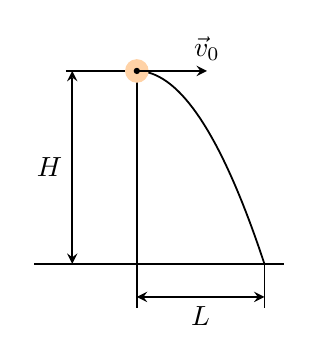
\begin{tikzpicture}[>=stealth,line width=.65pt]
\draw (-1.3,0)--(1.87,0);
\draw (0,-.56)--(0,2.45);
\draw (1.62,0)--(1.62,-.56);
\draw[<->] (-.82,0)--(-.82,2.45) node[midway,left]{$H$};
\draw (-.9,2.45)--(0,2.45);
\draw[<->] (0,-.42)--(1.62,-.42) node[midway,below]{$L$};
\draw[domain=0:1.62,samples=35,smooth,variable=\x] plot ({\x},{2.45*(1-(\x/1.62)^2)});
\fill[orange!35] (0,2.45) circle (.15);
\fill (0,2.45) circle (.04);
\draw[->] (0,2.45)--(0.89,2.45) node[above]{$\vec v_0$};
\end{tikzpicture}
\end{center}
Шарик, брошенный горизонтально с высоты $H$ с начальной скоростью $\vec V_0,$ за время полета $t$ пролетел в горизонтальном направлении расстояние $L$ (см. рис.). Что произойдет с временем полета и ускорением шарика, если на той же установке при неизменной начальной скорости шарика увеличить высоту H? (Сопротивлением воздуха пренебречь.) 

Для каждой величины определите соответствующий характер ее изменения.

$1$. Увеличится.

$2$. Уменьшится.

$3$. Не изменится.

\begin{center}\small\renewcommand{\arraystretch}{1.25}\begin{tabular}{|p{0.450\linewidth}|p{0.450\linewidth}|}\hline
Время полета & Ускорение шарика\\\hline
 & \\\hline
\end{tabular}\end{center}
}{
\smallskip\noindent\textbf{Решение}\par
Вблизи поверхности Земли гравитационное поле можно считать однородным. Шарика падает с постоянным ускорением свободного падения. Время полета $T= \sqrt{\frac{2H}{g}}$ увеличивается с ростом высоты.

Ответ: $13$.
}

% Source sdamgia-10065: https://phys-ege.sdamgia.ru/problem?id=10065
\BankTask{sdamgia-10065}{
\begin{center}
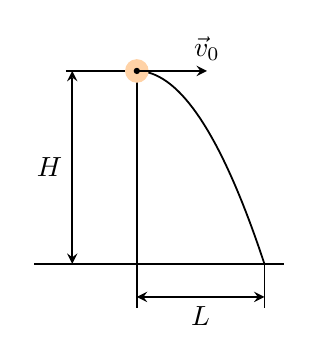
\begin{tikzpicture}[>=stealth,line width=.65pt]
\draw (-1.3,0)--(1.87,0);
\draw (0,-.56)--(0,2.45);
\draw (1.62,0)--(1.62,-.56);
\draw[<->] (-.82,0)--(-.82,2.45) node[midway,left]{$H$};
\draw (-.9,2.45)--(0,2.45);
\draw[<->] (0,-.42)--(1.62,-.42) node[midway,below]{$L$};
\draw[domain=0:1.62,samples=35,smooth,variable=\x] plot ({\x},{2.45*(1-(\x/1.62)^2)});
\fill[orange!35] (0,2.45) circle (.15);
\fill (0,2.45) circle (.04);
\draw[->] (0,2.45)--(0.89,2.45) node[above]{$\vec v_0$};
\end{tikzpicture}
\end{center}
Шарик, брошенный горизонтально с высоты $H$ с начальной скоростью $\vec v _0,$ до падения на землю пролетел в горизонтальном направлении расстояние $L$ (см. рис.). Что произойдет с временем полета до падения на землю и ускорением шарика, если на этой же установке увеличить начальную скорость шарика? Сопротивлением воздуха пренебречь.

Для каждой величины определите соответствующий характер изменения.

$1$. Увеличится.

$2$. Уменьшится.

$3$. Не изменится.

 

\begin{center}\small\renewcommand{\arraystretch}{1.25}\begin{tabular}{|p{0.450\linewidth}|p{0.450\linewidth}|}\hline
Время полета шарика до падения на землю & Ускорение шарика\\\hline
 & \\\hline
\end{tabular}\end{center}
}{
\smallskip\noindent\textbf{Решение}\par
Время полета шарика определяется временем его падения и рассчитывается по формуле $t= \sqrt{\frac{2H}{g}} .$ При увеличении начальной скорости время полета не изменится. 

Ускорение шарика постоянно и равно ускорению свободного падения.

Ответ: $33$.
}

% Source sdamgia-12856: https://phys-ege.sdamgia.ru/problem?id=12856
\BankTask{sdamgia-12856}{
Из точки, находящейся на высоте $101{,}25\,\text{м}$ над горизонтальной площадкой, брошено тело массой $1\,\text{кг}$, начальная скорость которого направлена по горизонтали. Тело движется в плоскости XOY, уравнение его траектории имеет вид: $y = 101{,}25 - 1{,}25x ^2 .$ В момент броска тело имело координату $x = 0\,\text{м}$. Установите соответствие между физическими величинами и их значениями в СИ. 

\TaskMatchingColumns{Физическая величина}{А) дальность полета тела\par 
Б) начальная кинетическая энергия тела}{Значение в си}{$1$) $1{,}25$\par 
$2$) $2$\par 
$3$) $9$\par 
$4$) $101{,}25$}

\begin{center}\small\renewcommand{\arraystretch}{1.25}\begin{tabular}{|p{0.450\linewidth}|p{0.450\linewidth}|}\hline
А & Б\\\hline
 & \\\hline
\end{tabular}\end{center}
}{
\smallskip\noindent\textbf{Решение}\par
Дальность полета можно найти, решив уравнение:

$y=0 \Longleftrightarrow  101{,}25 - 1{,}25x ^2 =0 \Longleftrightarrow  |x|=9\,\text{м}$ (А — $3$).

Время падения брошенного горизонтально тела составляет $\sqrt{\frac{2h}{g}}=\sqrt{\frac{2\cdot101{,}25}{10}}=4{,}5\,\text{с}.$ За это время тело пролетело по горизонтали $9\,\text{м}$, значит, горизонтальная проекция скорости равна $\frac{9}{4{,}5} = 2\,\text{м/с}.$ Таким образом, начальная кинетическая энергия тела $\frac{1 \cdot  2 ^2}{2} =2\,\text{Дж}$ (Б — $2$).

Ответ: $32$.
}

% Source sdamgia-25022: https://phys-ege.sdamgia.ru/problem?id=25022
\BankTask{sdamgia-25022}{
\begin{center}
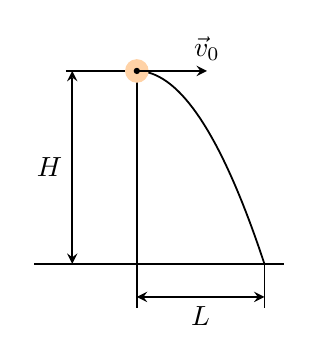
\begin{tikzpicture}[>=stealth,line width=.65pt]
\draw (-1.3,0)--(1.87,0);
\draw (0,-.56)--(0,2.45);
\draw (1.62,0)--(1.62,-.56);
\draw[<->] (-.82,0)--(-.82,2.45) node[midway,left]{$H$};
\draw (-.9,2.45)--(0,2.45);
\draw[<->] (0,-.42)--(1.62,-.42) node[midway,below]{$L$};
\draw[domain=0:1.62,samples=35,smooth,variable=\x] plot ({\x},{2.45*(1-(\x/1.62)^2)});
\fill[orange!35] (0,2.45) circle (.15);
\fill (0,2.45) circle (.04);
\draw[->] (0,2.45)--(0.89,2.45) node[above]{$\vec v_0$};
\end{tikzpicture}
\end{center}
Шарик массой $m$, брошенный горизонтально с высоты $H$ с начальной скоростью $\vec v _0,$ за время полета $t$ пролетел в горизонтальном направлении расстояние $L$ (см. рис.). В другом опыте на этой же установке шарик массой $0{,}5$m бросают с той же высоты со скоростью $2\vec v _0.$ Что произойдет во втором опыте с дальностью полета и временем полета шарика по сравнению с первым опытом? Сопротивлением воздуха пренебречь. 

Для каждой величины определите соответствующий характер ее изменения.

$1$. Увеличится.

$2$. Уменьшится.

$3$. Не изменится.

 

\begin{center}\small\renewcommand{\arraystretch}{1.25}\begin{tabular}{|p{0.450\linewidth}|p{0.450\linewidth}|}\hline
Дальность полета

шарика & Время полета

шарика\\\hline
 & \\\hline
\end{tabular}\end{center}
}{
\smallskip\noindent\textbf{Решение}\par
Время полета найдем из формулы высоты, с которой тело брошено горизонтально: 

\[h= \frac{gt ^2}{2} \Rightarrow t= \sqrt{\frac{2h}{g}} .\]

Время полета не зависит ни от массы, ни от начальной скорости, значит, не изменится ($3$).

Дальность полета тела, брошенного горизонтально, равно $L= v _0t.$ Следовательно, при увеличении скорости увеличивается и дальность полета ($1$).

Ответ: $13$.
}

% Source sdamgia-38188: https://phys-ege.sdamgia.ru/problem?id=38188
\BankTask{sdamgia-38188}{
\begin{center}
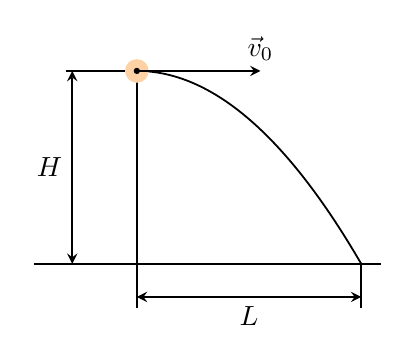
\begin{tikzpicture}[>=stealth,line width=.65pt]
\draw (-1.3,0)--(3.1,0);
\draw (0,-.56)--(0,2.45);
\draw (2.85,0)--(2.85,-.56);
\draw[<->] (-.82,0)--(-.82,2.45) node[midway,left]{$H$};
\draw (-.9,2.45)--(0,2.45);
\draw[<->] (0,-.42)--(2.85,-.42) node[midway,below]{$L$};
\draw[domain=0:2.85,samples=35,smooth,variable=\x] plot ({\x},{2.45*(1-(\x/2.85)^2)});
\fill[orange!35] (0,2.45) circle (.15);
\fill (0,2.45) circle (.04);
\draw[->] (0,2.45)--(1.57,2.45) node[above]{$\vec v_0$};
\end{tikzpicture}
\end{center}
Шарик, брошенный горизонтально с высоты $H$ с начальной скоростью $\vec v _0,$ за время $t$ пролетел в горизонтальном направлении расстояние $L$ (см. рис.). Как изменятся дальность полёта $L$ и скорость шарика в момент падения, если, не меняя начальной скорости шарика, увеличить высоту H? Сопротивлением воздуха пренебречь.

Для каждой величины определите соответствующий характер изменения:

$1$) увеличится

$2$) уменьшится

$3$) не изменится

 

\begin{center}\small\renewcommand{\arraystretch}{1.25}\begin{tabular}{|p{0.450\linewidth}|p{0.450\linewidth}|}\hline
Дальность полета & Скорость шарика

в момент падения\\\hline
 & \\\hline
\end{tabular}\end{center}
}{
\smallskip\noindent\textbf{Решение}\par
Движение шарика при отсутствии силы сопротивления происходит только под действием силы тяжести, а следовательно, с ускорением свободного падения $g$, направленным вертикально вниз. Поэтому движение тела по оси Ox является равномерным, а по оси Oy — равноускоренным без начальной скорости (так как $v_{0y}=0$). Тогда $H = \frac{gt ^2}{2} ,$ $L= v _0t.$

Тогда при увеличении высоты броска время движения шарика увеличится, соответственно, увеличится и дальность полета ($1$).

Скорость шарика в момент падения $v = \sqrt{v _x ^2 + v _y ^2} .$ При этом $v _x= v _0,$ $a$ $v _y=gt,$ то, учитывая, что время движения увеличится, делаем вывод, что скорость шарика в момент падения увеличится ($1$).

Ответ: $11$.
}

% Source sdamgia-52033: https://phys-ege.sdamgia.ru/problem?id=52033
\BankTask{sdamgia-52033}{
Мячик брошен горизонтально с края крыши дома. Как изменятся модуль скорости мячика при его падении на землю и его ускорение в течение полёта, если бросить мячик с той же начальной скоростью из той же точки вверх под углом $30^\circ$ к горизонту? Сопротивлением воздуха пренебречь, дом стоит на горизонтальной площадке.

Для каждой величины определите соответствующий характер ее изменения.

$1$. Увеличится.

$2$. Уменьшится.

$3$. Не изменится.

 

\begin{center}\small\renewcommand{\arraystretch}{1.25}\begin{tabular}{|p{0.450\linewidth}|p{0.450\linewidth}|}\hline
Модуль скорости мячика при его падении на землю & Ускорение мячика\\\hline
 & \\\hline
\end{tabular}\end{center}
}{
\smallskip\noindent\textbf{Решение}\par
При обоих вариантах движения выполняется закон сохранения энергии $E_{\text{п}}1 + E_{\text{к}}1 = E_{\text{к}}2.$ Так как высота, с которой брошено тело, и начальная скорость одинаковы, то полная энергия тела в момент броска одинакова в обоих случаях. Следовательно, в момент падения тела обладали одинаковой кинетической энергией и соответственно одинаковой скоростью ($3$).

В обоих случаях мяч двигался с ускорением свободного падения, которое не менялось ($3$).

Ответ: $33$.
}

% Source sdamgia-4498: https://phys-ege.sdamgia.ru/problem?id=4498
\BankTask{sdamgia-4498}{
Дом стоит на краю поля. С балкона с высоты $5\,\text{м}$ мальчик бросил камешек в горизонтальном направлении. Начальная скорость камешка $7\,\text{м/с}$, его масса $0{,}1\,\text{кг}$. Какова кинетическая энергия камешка через $2\,\text{с}$ после броска?
}{
\smallskip\noindent\textbf{Решение}\par
Тело, брошенное горизонтально, движется под действием силы тяжести с ускорением свободного падения, направленным вертикально вниз. При этом: $g_x=0,g_y= - g,$ то есть по оси $0x$ движение равномерное со скоростью $v _x= v _0,$ по оси $0y$ движение равноускоренное с начальной скоростью $v _{0y}=0.$

Следовательно, при равноускоренном движении вертикальное перемещение равно $h = \frac{gt ^2}{2} ,$ откуда время падения камешка

\[t= \sqrt{\frac{2h}{g}} = \sqrt{\frac{2 \cdot  5\,\text{м}}{10\,\text{м/с} ^2}} =1\,\text{с}.\]

При попадании в мягкую землю камешек застрянет в ней и остановится. Следовательно, через $2\,\text{с}$ после броска его скорость будет равна нулю, а значит, нулю будет равна и его кинетическая энергия.

Ответ: $0\,\text{Дж}$.
}

% Source sdamgia-46131: https://phys-ege.sdamgia.ru/problem?id=46131
\BankTask{sdamgia-46131}{
Камень брошен горизонтально с высоты $H = 20\,\text{м}$ над поверхностью земли. Определите, под каким углом $\alpha $ к горизонту был направлен вектор скорости камня в момент удара о землю, если дальность его полета равна s = $15\,\text{м}$. Сопротивлением воздуха пренебречь.
}{
\smallskip\noindent\textbf{Решение}\par
$1$. Выберем инерциальную систему отсчёта, связанную с землёй. Направим ось Ox горизонтально в направлении вектора начальной скорости камня, а ось Oy — вертикально вниз. Тогда проекции начальной скорости камня и ускорения свободного падения на эти оси будут равны: $v _{0x} = v _0,$ $v _{0y} = 0,$ $g_x = 0,$ $g_y = g.$

$2$. В момент падания камня на землю вектор его скорости направлен под углом $\alpha $ к горизонту. Вектор скорости и его проекции на оси Ox и Oy образуют прямоугольный треугольник. Тангенс угла наклона к горизонту равен: $\tan  \alpha  = \frac{v _y}{v _x} .$

$3$. Вертикальная проекция скорости $v _y,$ меняющаяся со временем линейно, в выбранной системе отсчёта принимает значение $v _y = v _{0y} + gt = gt,$ где $t$ — время падения камня. Горизонтальная составляющая скорости при этом равна $v _x = v _{0x} = v _0.$ Следовательно, $\tan  \alpha  = \frac{gt}{v _0} .$

$4$. Высота, с которой был брошен камень, равна $H = \frac{gt ^2}{2} ,$ а дальность полета $s = v _0 t.$

$5$. Используя записанные уравнения, окончательно получим: 

\[\tan  \alpha  = \frac{2H}{s} = \frac{2 \cdot  20}{15} = \frac{8}{3} ,\]

\[\alpha  = \arctan  \frac{8}{3} \approx 70 ^\circ.\]

Ответ: $\alpha  \approx 70 ^\circ.$
}


% Source 25945: https://phys-ege.sdamgia.ru/problem?id=25945
\BankTask{25945}{
Пушка, закрепленная на высоте $5\,\text{м}$, стреляет в горизонтальном направлении снарядами массой $10\,\text{кг}$. Вследствие отдачи ее ствол сжимает на $1\,\text{м}$ пружину жесткостью $6$ · $10^{3}$ Н/м, производящую перезарядку пушки. При этом на сжатие пружины идет относительная доля $\eta = \frac{1}{6}$ энергии отдачи. Какова масса ствола, если дальность полета снаряда равна $600\,\text{м}$? Сопротивлением воздуха при полете снаряда пренебречь.
Какие законы Вы используете для описания взаимодействия пушки и снаряда и дальнейшего движения тел? Обоснуйте их применение к данному случаю.
}{
\smallskip\noindent\textbf{Решение}\par
Обоснование
Систему отсчета, связанную с Землей, будем считать инерциальной. Между снарядом и пушкой происходит взаимодействие через давление пороховых газов. Поскольку внутренние силы давления пороховых газов достаточно велики, так как промежуток времени взаимодействия мал, а импульс каждого из тел изменяется на конечную величину, то действием внешних сил трения, тяжести и реакции опоры можно пренебречь по сравнению с силами давления пороховых газов. Значит, в ИСО можно применить закон сохранения импульса.
При отдаче пушка приобретает кинетическую энергию, которая частично переходит в потенциальную энергию упруго деформированной пружины. В инерциальной системе отсчета можно применить закон превращения энергии, поскольку действие непотенциальных сил на тело пренебрежимо мало. Причем потенциальная энергия взаимодействия с Землей не изменяется, так как платформа горизонтальна.
Движение снаряда после взаимодействия можно считать поступательным, поэтому снаряд является материальной точкой. На него действует только сила тяжести, которая является причиной ускорения свободного падения, направленного вертикально вниз. Следовательно, применимы законы прямолинейного равноускоренного движения по оси 0y и прямолинейного равномерного движения по оси 0x.

Перейдем к решению. 
Пусть $v _{\,\text{п}}, v _c$  — соответственно начальные скорости пушки и снаряда, $m_{\,\text{п}},m_c$  — массы пушки и снаряда. Энергия сжатой пружины равна $\frac{kx ^2}{2} ,$ где $x$  — сжатие пружины, $k$  — жесткость пружины. Энергия отдачи пушки равна $\frac{m_{\,\text{п}} v _{\,\text{п}} ^2}{2} = \frac{kx ^2}{2\eta} ,$ откуда $m_{\,\text{п}} = \frac{kx ^2}{v _{\,\text{п}} ^2 \eta} .$ 
Найдем начальную скорость пушки. Для этого воспользуемся законом сохранения импульса: $m_{\,\text{п}} v _{\,\text{п}} = m_{\,\text{с}} v _{\,\text{с}},$ откуда $v _{\,\text{п}} = \frac{m_{\,\text{с}}}{m_{\,\text{п}}} v _{\,\text{с}}.$ Значит, $m_{\,\text{п}} = \frac{kx ^2 m_{\,\text{п}} ^2}{v _{\,\text{с}} ^2 m_{\,\text{с}} ^2 \eta} ,$ откуда $m_{\,\text{п}} = \frac{v _{\,\text{с}} ^2 m_{\,\text{с}} ^2 \eta}{kx ^2} .$
На снаряд действует только сила тяжести поэтому время падения t и высота $h$, с которой он падает связаны формулой: $h = \frac{gt ^2}{2} ,$ откуда $t = \sqrt{\frac{2h}{g}} .$ После выстрела на снаряд вдоль горизонтальной оси не действуют никакие силы, поэтому дальность полета снаряда $L$ связана с горизонтальной составляющей скорости $v _x$ равенством $L = v _x t.$ Заметим, что $v _x = v _{\,\text{с}},$ поэтому $v _{\,\text{с}} = \frac{L}{t} = \sqrt{\frac{g}{2h}} L.$ 
Подставим выражение для скорости снаряда в выражение для массы пушки: $m_{\,\text{п}} = \frac{g}{2h} L ^2 \cdot \frac{m_{\,\text{с}} ^2 \eta}{kx ^2} .$ 
Подставив числовые значения в выражение, получим $m_{\,\text{п}}= \frac{10 \cdot 600 ^2 \cdot 10 ^2}{6 \cdot 2 \cdot 5 \cdot 6 \cdot 10 ^3 \cdot 1} = 1000\,\text{кг}.$

Ответ: $1000\,\text{кг}$.
}

\end{document}
